\documentclass{article}

\usepackage{placeins}
\usepackage{amsmath}
\usepackage{amssymb}
\usepackage{graphicx}
\usepackage{geometry}
\usepackage{setspace}
\usepackage{parskip}
\usepackage{float}
\usepackage{booktabs}
\usepackage{hyperref}

\geometry{margin=1in}
\setstretch{1.15}

\hypersetup{
    colorlinks=true,
    linkcolor=blue
}

\begin{document}

% =================================================
% Title Page
% =================================================

\begin{titlepage}

\begin{flushright}
    % Add the TU Wien logo file here if available.
\end{flushright}

\vspace{1cm}

\begin{center}
    {\LARGE \textbf{Machine Learning Algorithms}}\\[0.5cm]
    {\Large Course Code: 389.204}\\[0.5cm]
    {\large Technische Universit\"at Wien}\\
    {\large Institute of Telecommunications}\\
    {\large Faculty of Electrical Engineering and Information Technology}
\end{center}

\vspace{1.5cm}

\begin{center}
    \Large\textbf{Submission of Exercise 3}
\end{center}

\vspace{1cm}

\begin{center}
\begin{tabular}{rl}
    \textbf{Name:} & Pol Andreu Lomas\\
    \\[0.2cm]
    \textbf{Student ID:} & 54923214L \\
    \\[0.2cm]
    \textbf{Submission Date:} & 15.05.2026 \\
\end{tabular}
\end{center}

\vfill

\section*{Integrity Statement}

I hereby declare that the work presented in this assignment/report is my own and has been prepared without any unauthorized assistance. I confirm that I have fully acknowledged and referenced all sources used.

\vspace{2cm}

\noindent\textbf{Signature:} \underline{\hspace{6cm}}

\end{titlepage}

% =================================================
% Problem 3.1
% =================================================

\section*{Problem 3.1}

\subsection*{3.1.1 XOR}

\textbf{Task:} Configure the network such that it implements the XOR function using suitable activations, weights, and biases.

\vspace{0.3cm}

\textbf{Results:}

\begin{table}[H]
\centering
\caption{Network activations and outputs.}

\begin{tabular}{cccccccc}
\toprule
\(\mathbf{x}^\top\) &
\(y\) &
\(a_0^{(0)}\) &
\(z_0^{(0)}\) &
\(a_1^{(0)}\) &
\(z_1^{(0)}\) &
\(a_0^{(1)}\) &
\(\hat{y}\) \\
\midrule
\([0,0]\) & 0 & 0  & 0 & 0  & 0 & 0 & 0 \\
\([0,1]\) & 1 & 1  & 1 & -1 & 0 & 1 & 1 \\
\([1,0]\) & 1 & -1 & 0 & 1  & 1 & 1 & 1 \\
\([1,1]\) & 0 & 0  & 0 & 0  & 0 & 0 & 0 \\
\bottomrule
\end{tabular}

\end{table}

The hidden layer was designed such that each ReLU neuron activates only for one of the two valid XOR cases. Specifically, the first neuron detects \([0,1]\) through \(a_0^{(0)} = -x_0 + x_1\), while the second neuron detects \([1,0]\) through \(a_1^{(0)} = x_0 - x_1\).

The output neuron then performs a simple linear sum of both hidden activations, producing an output of 1 whenever exactly one hidden neuron is active, which reproduces the XOR function.

% -------------------------------------------------

\subsection*{3.1.2 Chain Rule}

\textbf{Task:} Derive the gradients of

\[
L(w,b) = (y-\hat{y})^2
\]

using the chain rule and briefly explain why backpropagation is computationally efficient.

\vspace{0.3cm}

\textbf{Results:}

To determine how the loss changes with respect to a weight, we apply the chain rule through every intermediate dependency between that weight and the loss. For the output layer weights, the dependency chain is short since the weights directly affect the prediction. For hidden-layer weights, the gradient must propagate through all following neurons until reaching the loss function.

For the output neuron with linear activation,

\[
\hat{y} = a_0^{(1)}
\]

the derivative of the loss with respect to the prediction is

\[
\frac{\partial L}{\partial \hat{y}} = 2(\hat{y}-y).
\]

For the output layer weight \(w_{0,0}^{(1)}\),

\[
\frac{\partial L}{\partial w_{0,0}^{(1)}}
=
\frac{\partial L}{\partial \hat{y}}
\cdot
\frac{\partial \hat{y}}{\partial w_{0,0}^{(1)}}
=
2(\hat{y}-y)z_0^{(0)}.
\]

For a hidden-layer weight such as \(w_{0,0}^{(0)}\), the dependency chain becomes

\[
w_{0,0}^{(0)}
\rightarrow
a_0^{(0)}
\rightarrow
z_0^{(0)}
\rightarrow
a_0^{(1)}
\rightarrow
\hat{y}
\rightarrow
L.
\]

Applying the chain rule gives

\[
\frac{\partial L}{\partial w_{0,0}^{(0)}}
=
\frac{\partial L}{\partial \hat{y}}
\cdot
\frac{\partial \hat{y}}{\partial a_0^{(1)}}
\cdot
\frac{\partial a_0^{(1)}}{\partial z_0^{(0)}}
\cdot
\frac{\partial z_0^{(0)}}{\partial a_0^{(0)}}
\cdot
\frac{\partial a_0^{(0)}}{\partial w_{0,0}^{(0)}}.
\]

If linear activations are used, then

\[
\frac{\partial z}{\partial a}=1,
\]

while for nonlinear activations such as ReLU,

\[
\frac{\partial z}{\partial a}=\sigma'(a)
\]

must also be included in the chain rule.

Backpropagation is computationally efficient because intermediate gradients can be reused for multiple parameters instead of being recomputed independently. Once the gradient at one layer is known, it can be propagated backwards through the network to efficiently compute the gradients of all previous layers.

% -------------------------------------------------

\subsection*{3.1.3 NN Implementation}

\textbf{Task:} Implement the network in JAX, train it for the logical AND operation, and report the learned parameters.

\vspace{0.3cm}

\textbf{Results:}

\begin{table}[H]
\centering
\caption{Learned weights and biases after training for logical AND.}

\begin{tabular}{cc}
\toprule
Parameter & Value \\
\midrule
\(W^{(0)}\) &
\(
\begin{bmatrix}
0.7783 & -2.5447 \\
-2.4330 & -0.9102
\end{bmatrix}
\)
\\[0.5cm]

\(b^{(0)}\) &
\(
\begin{bmatrix}
1.6534 \\
3.4537
\end{bmatrix}
\)
\\[0.5cm]

\(W^{(1)}\) &
\(
\begin{bmatrix}
-3.0394 \\
-4.3703
\end{bmatrix}
\)
\\[0.5cm]

\(b^{(1)}\) &
\(
\begin{bmatrix}
4.4403
\end{bmatrix}
\)
\\

\bottomrule
\end{tabular}

\end{table}

% =================================================
% Problem 3.2
% =================================================

\section*{Problem 3.2}

\subsection*{3.2.1 Flax Models}

\textbf{Task:} Implement the baseline and dropout architectures in Flax using ReLU hidden activations and softmax outputs.

\vspace{0.3cm}

\textbf{Results:}

Both models were implemented using the same three-hidden-layer MLP structure with hidden sizes \((128,128,128)\), and the dropout model used a dropout rate of \(0.5\) after each hidden layer. The trainable parameter count of a dense layer is

\[
\text{parameters} = (\text{input dimension} \times \text{output dimension}) + \text{output dimension},
\]

where the first term corresponds to the weights and the second to the biases. For example, a dense layer mapping \(128 \rightarrow 128\) contains

\[
128 \times 128 + 128 = 16512
\]

trainable parameters.

Dropout layers do not add trainable parameters because they only apply a random masking operation during training, temporarily deactivating some neurons. Therefore, the number of trainable parameters is unchanged; dropout only modifies the effective computation during each forward pass.

% -------------------------------------------------

\subsection*{3.2.2 Dataset and DataModule}

\textbf{Task:} Load \texttt{classification.csv}, one-hot encode the labels, split the dataset, and implement mini-batch loading.

\vspace{0.3cm}

\textbf{Results:}

The dataset contains 5000 samples with 11 input features and 3 classes. The targets were converted to one-hot encoding, the data was split using \texttt{train\_test\_split} with \texttt{test\_size=0.3} and \texttt{random\_state=0}, and the features were standardized using \texttt{StandardScaler}. The resulting shapes were:

\[
X_{\text{train}} \in \mathbb{R}^{3500 \times 11}, \qquad X_{\text{test}} \in \mathbb{R}^{1500 \times 11}.
\]

Mini-batches of size 64 were yielded by the implemented \texttt{DataModule}, together with a mask for the padded last batch.

% -------------------------------------------------

\subsection*{3.2.3 Adam Optimizer}

\textbf{Task:} Train both models for 200 epochs using Adam and compare train/test accuracy.

\vspace{0.3cm}

\textbf{Results:}

\begin{table}[H]
\centering
\caption{Training and test accuracy.}
\begin{tabular}{lcc}
\toprule
Model & Train Accuracy & Test Accuracy \\
\midrule
Baseline & 0.9957 & 0.8307 \\
Dropout & 0.8960 & 0.8840 \\
\bottomrule
\end{tabular}
\end{table}

The dropout model achieved the higher accuracy on \(T_{test}\). The baseline network fit the training data almost perfectly, but this was accompanied by a noticeably lower test accuracy. In contrast, dropout reduced the training accuracy while improving generalization, indicating that the baseline model was overfitting and that regularization was beneficial for this dataset.

% -------------------------------------------------

\subsection*{3.2.4 Learning Curves}

\textbf{Task:} Track train/test loss and accuracy during training and analyze the learning curves.

\vspace{0.3cm}

\textbf{Results:}

The learning curves showed that the baseline model rapidly increased its training accuracy while the gap to test accuracy remained substantial, which is a typical sign of overfitting. The dropout model learned more slowly, but the training and test curves remained closer together and the final test accuracy was higher. Hence, the main effect of dropout in this exercise was to reduce overfitting and improve generalization.

% -------------------------------------------------

\subsection*{3.2.5 Early Stopping}

\textbf{Task:} Implement early stopping using validation accuracy.

\vspace{0.3cm}

\textbf{Results:}

\begin{figure}[H]
\centering
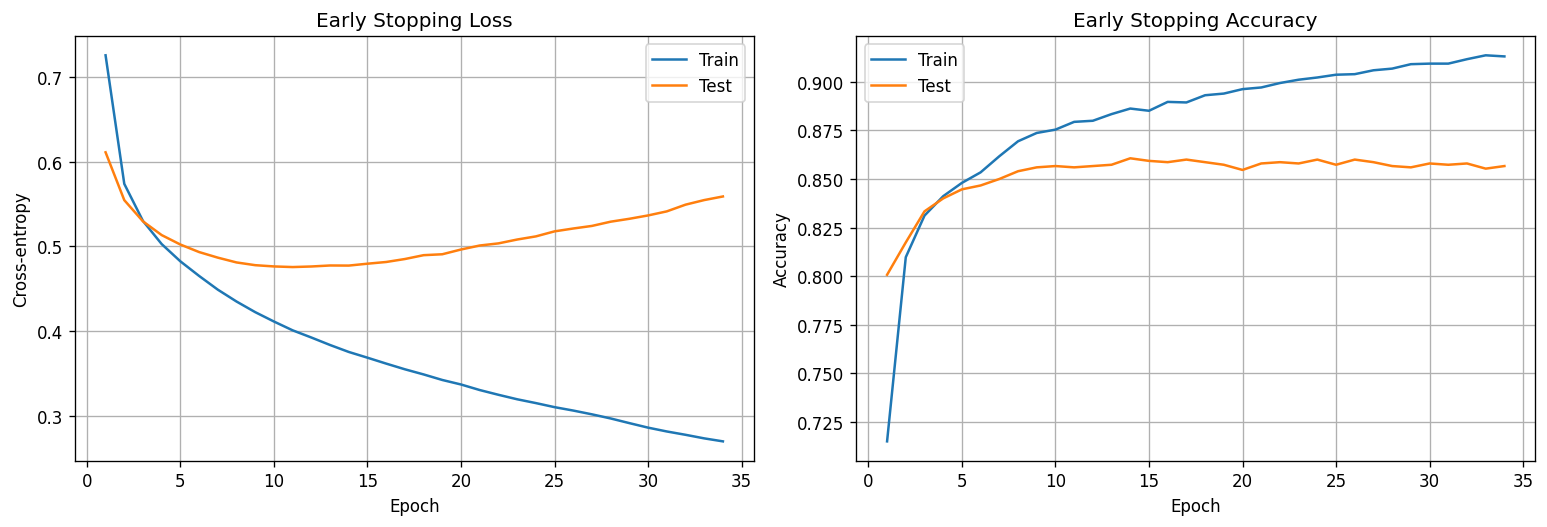
\includegraphics[width=\textwidth]{3.2.5.png}
\caption{Early stopping learning curves for the baseline model.}
\end{figure}

Early stopping was implemented with \texttt{min\_delta = 10^{-3}} and \texttt{patience = 20}. Training stopped after 34 epochs, and the best validation state was restored before evaluation. The restored model achieved a test accuracy of 0.8607, which is an improvement over the baseline model without early stopping (0.8307). This confirms that the original baseline model kept fitting the training data after the validation accuracy had already saturated.

% -------------------------------------------------

\subsection*{3.2.6 California Housing}

\textbf{Task:} Train a neural network achieving MAE \(<0.35\) on the California Housing dataset.

\vspace{0.3cm}

\textbf{Results:}

\begin{figure}[H]
\centering
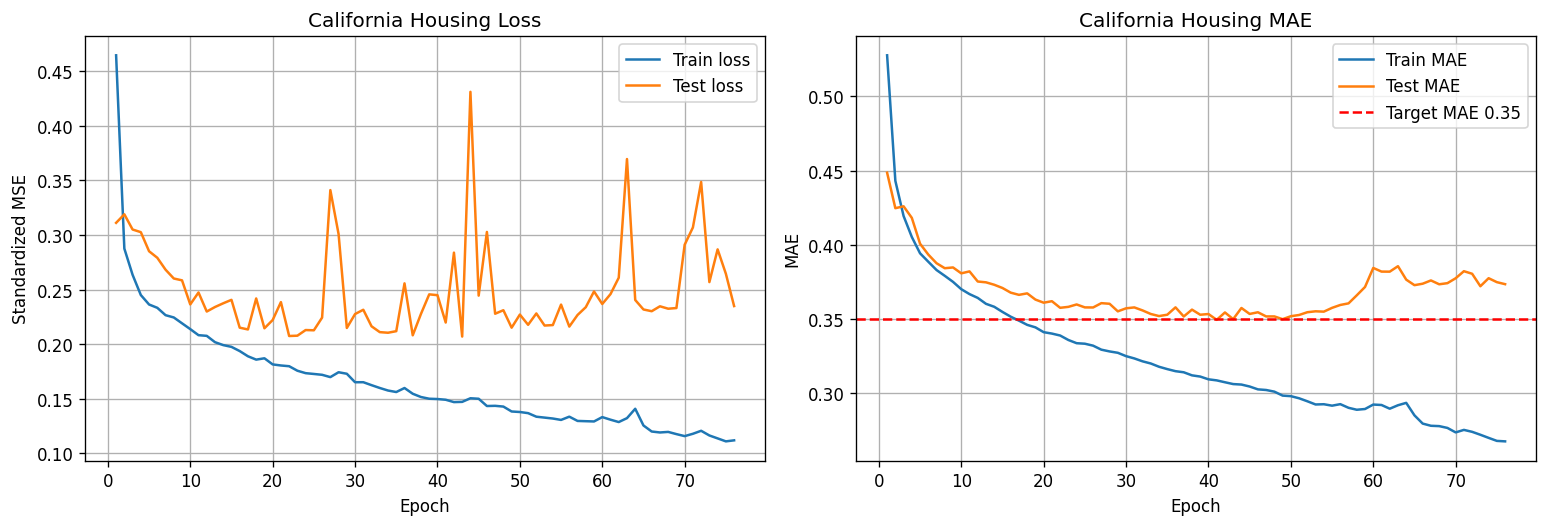
\includegraphics[width=\textwidth]{3.2.6.png}
\caption{Learning curves for California Housing regression.}
\end{figure}

The final model used standardized inputs, standardized targets during training, three hidden layers with sizes \((256,256,128)\), ReLU activations, the AdamW optimizer with learning rate \(10^{-3}\), weight decay \(10^{-5}\), and gradient clipping with norm 1.0. The resulting test MAE was

\[
\mathrm{MAE}_{\text{test}} = 0.3494,
\]

which satisfies the exercise requirement of staying below 0.35.

% =================================================
% Problem 3.3
% =================================================

\section*{Problem 3.3}

\subsection*{3.3.1 Probabilistic Loss}

\textbf{Task:} Expand the Gaussian negative log-likelihood and derive gradients with respect to \(\mu_\theta\) and \(\sigma_\theta\).

\vspace{0.3cm}

\textbf{Results:}

For a scalar Gaussian output, the negative log-likelihood can be written as

\[
J_y(\mu_\theta,\sigma_\theta)
=
\frac{1}{2}\log(2\pi)
+
\log(\sigma_\theta)
+
\frac{(y-\mu_\theta)^2}{2\sigma_\theta^2}.
\]

The gradient with respect to the predicted mean is

\[
\frac{\partial J_y}{\partial \mu_\theta}
=
\frac{\mu_\theta-y}{\sigma_\theta^2}.
\]

This gradient becomes zero when the prediction is exact, i.e. when \(\mu_\theta = y\). It is scaled by the inverse variance, so large predicted uncertainties reduce the update magnitude for the mean.

The gradient with respect to the predicted standard deviation is

\[
\frac{\partial J_y}{\partial \sigma_\theta}
=
\frac{1}{\sigma_\theta}
-
\frac{(y-\mu_\theta)^2}{\sigma_\theta^3}.
\]

This gradient is zero when the predicted uncertainty matches the squared prediction error. Therefore, the network is encouraged to increase \(\sigma_\theta\) in regions with large errors and reduce it where the predictions are reliable.

% -------------------------------------------------

\subsection*{3.3.2 Deterministic Regression}

\textbf{Task:} Train a deterministic neural network with MSE loss and visualize predictions and errors.

\vspace{0.3cm}

\textbf{Results:}

\begin{figure}[H]
\centering
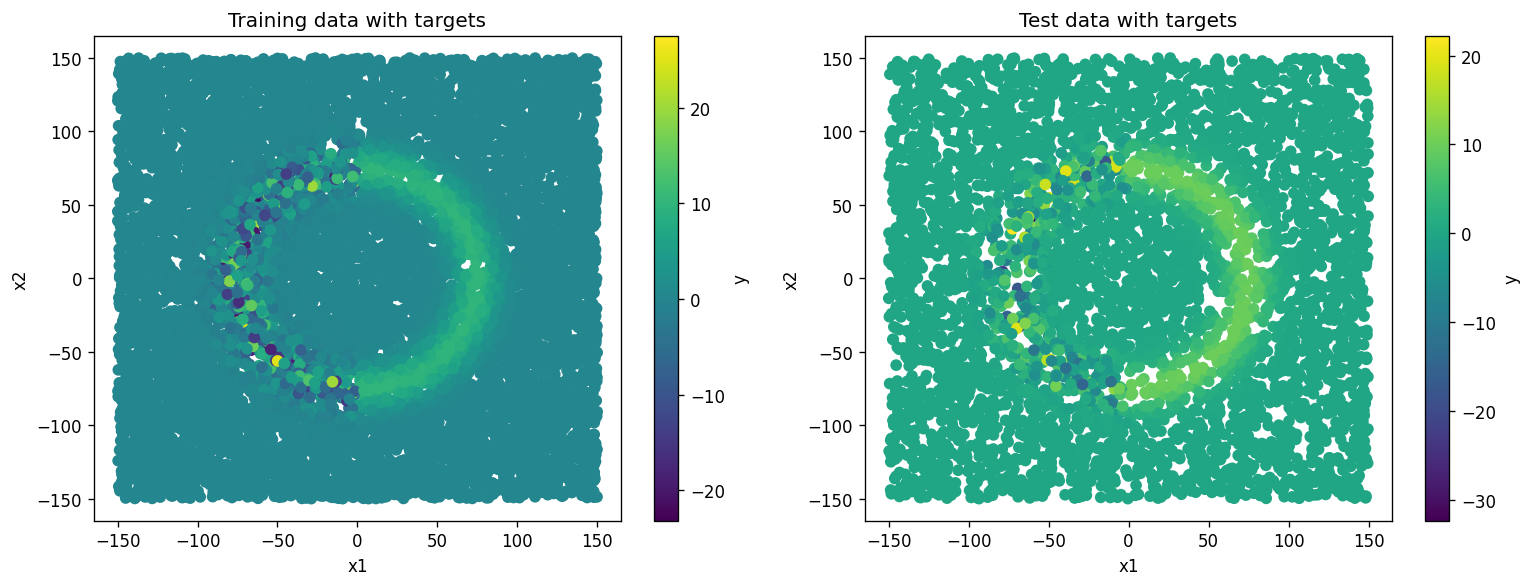
\includegraphics[width=\textwidth]{3.3.2.png}
\caption{Training and test samples of the \texttt{data\_uncertainty} dataset, colored by target value.}
\end{figure}

\begin{figure}[H]
\centering
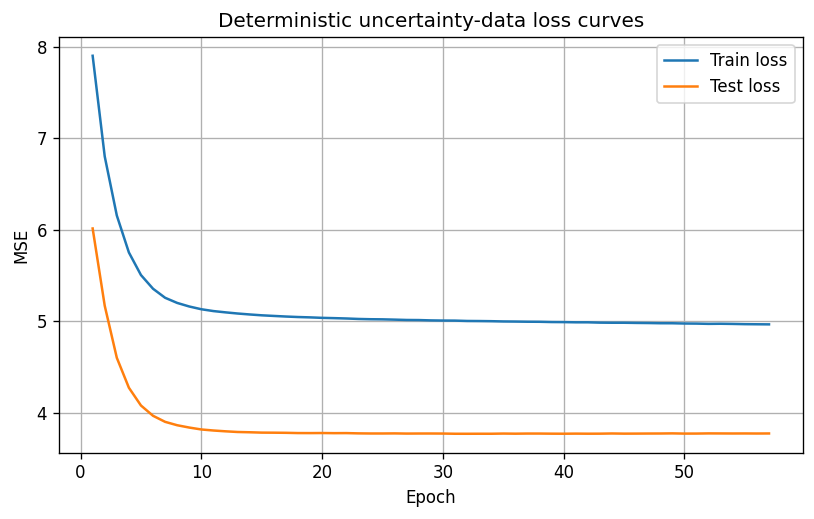
\includegraphics[width=0.85\textwidth]{3.3.2_3.png}
\caption{Learning curves of the deterministic model trained with MSE loss.}
\end{figure}

\begin{figure}[H]
\centering
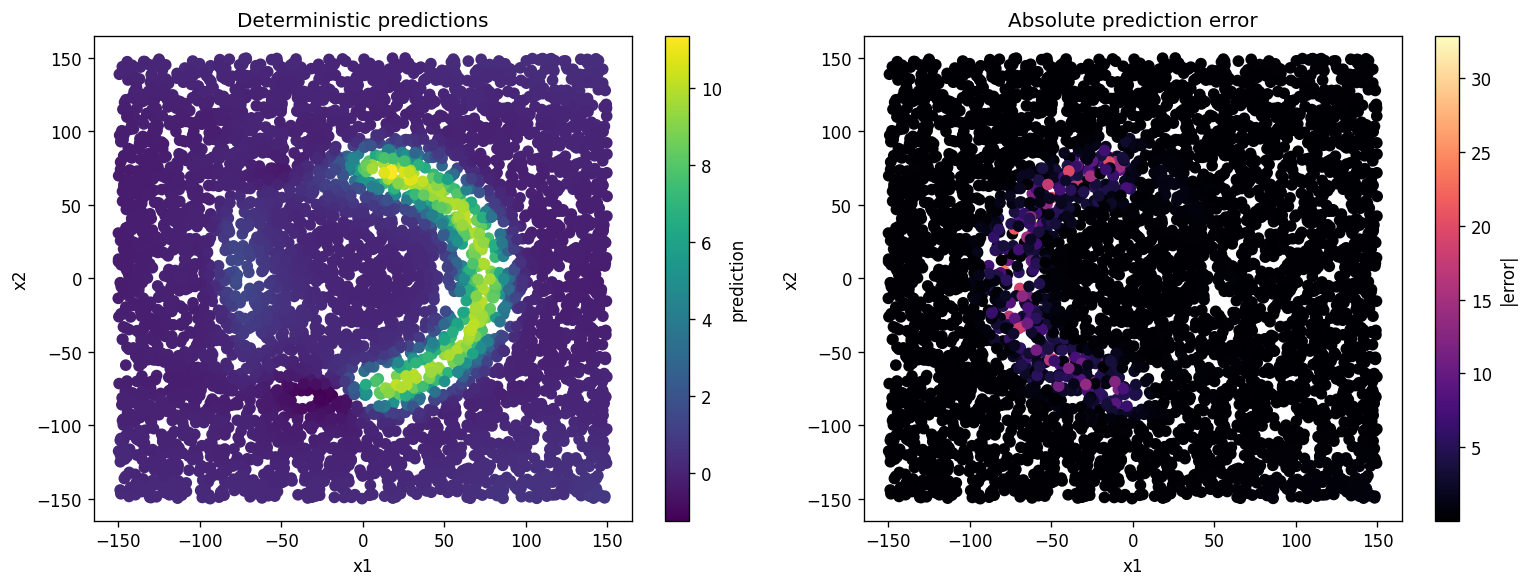
\includegraphics[width=\textwidth]{3.3.2_2.png}
\caption{Deterministic predictions and absolute prediction errors on the test set.}
\end{figure}

The deterministic two-hidden-layer network achieved a test MSE of 3.7702. The prediction plot shows that the model captures the broad structure of the target manifold, while the error plot indicates that the largest deviations occur mainly along the more difficult curved region of the dataset.

% -------------------------------------------------

\subsection*{3.3.3 Probabilistic Regression}

\textbf{Task:} Extend the model to predict both mean and uncertainty.

\vspace{0.3cm}

\textbf{Results:}

The output layer was extended to produce two values per sample: one for the predictive mean \(\mu_\theta\) and one for the log-variance. The standard deviation is recovered via

\[
\sigma_\theta = \exp\!\left(\frac{1}{2}\log\sigma_\theta^2\right),
\]

which guarantees a valid positive uncertainty value. The probabilistic model therefore predicts both an estimate and a sample-wise confidence level, and the negative log-likelihood from Section 3.3.1 is used as the training objective.

% -------------------------------------------------

\subsection*{3.3.4 Uncertainty Estimation}

\textbf{Task:} Train the probabilistic model and visualize predicted means and uncertainties.

\vspace{0.3cm}

\textbf{Results:}

\begin{figure}[H]
\centering
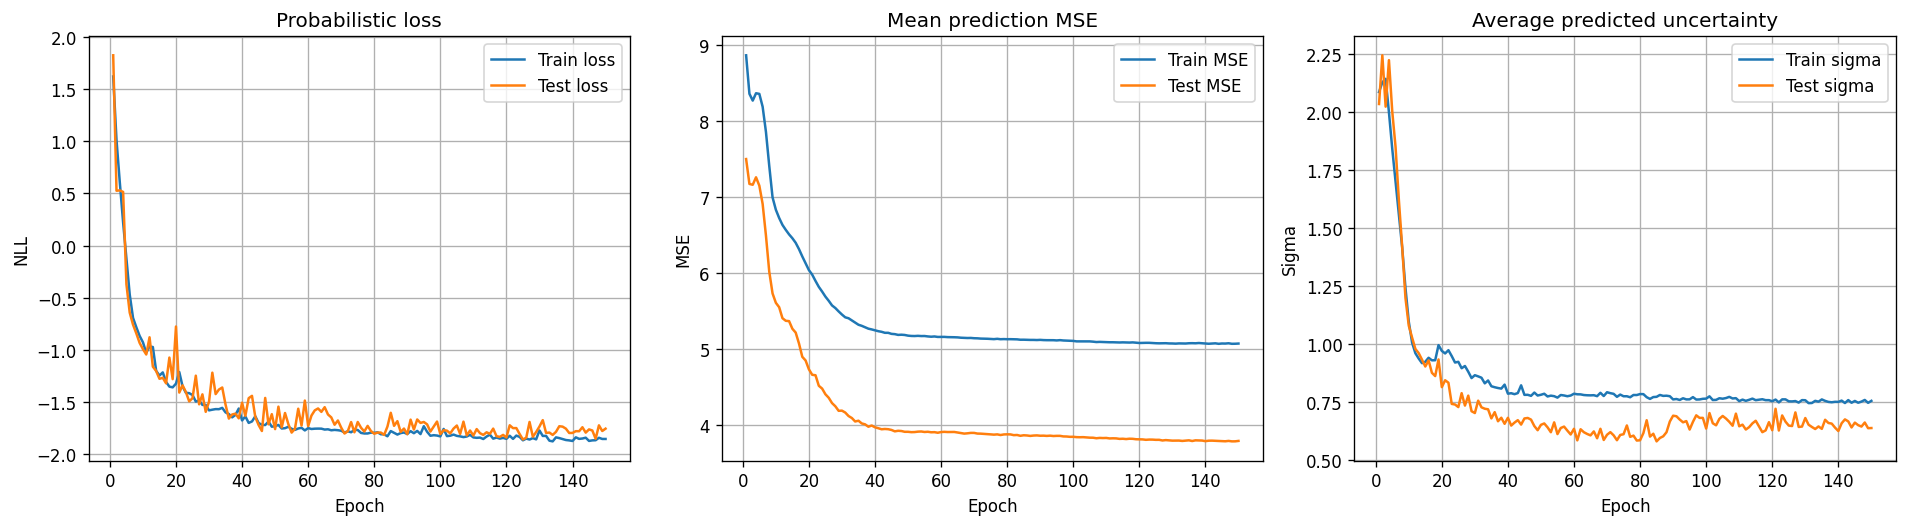
\includegraphics[width=\textwidth]{3.3.4.png}
\caption{Learning curves of the probabilistic model: NLL, MSE of the mean prediction, and average predicted uncertainty.}
\end{figure}

\begin{figure}[H]
\centering
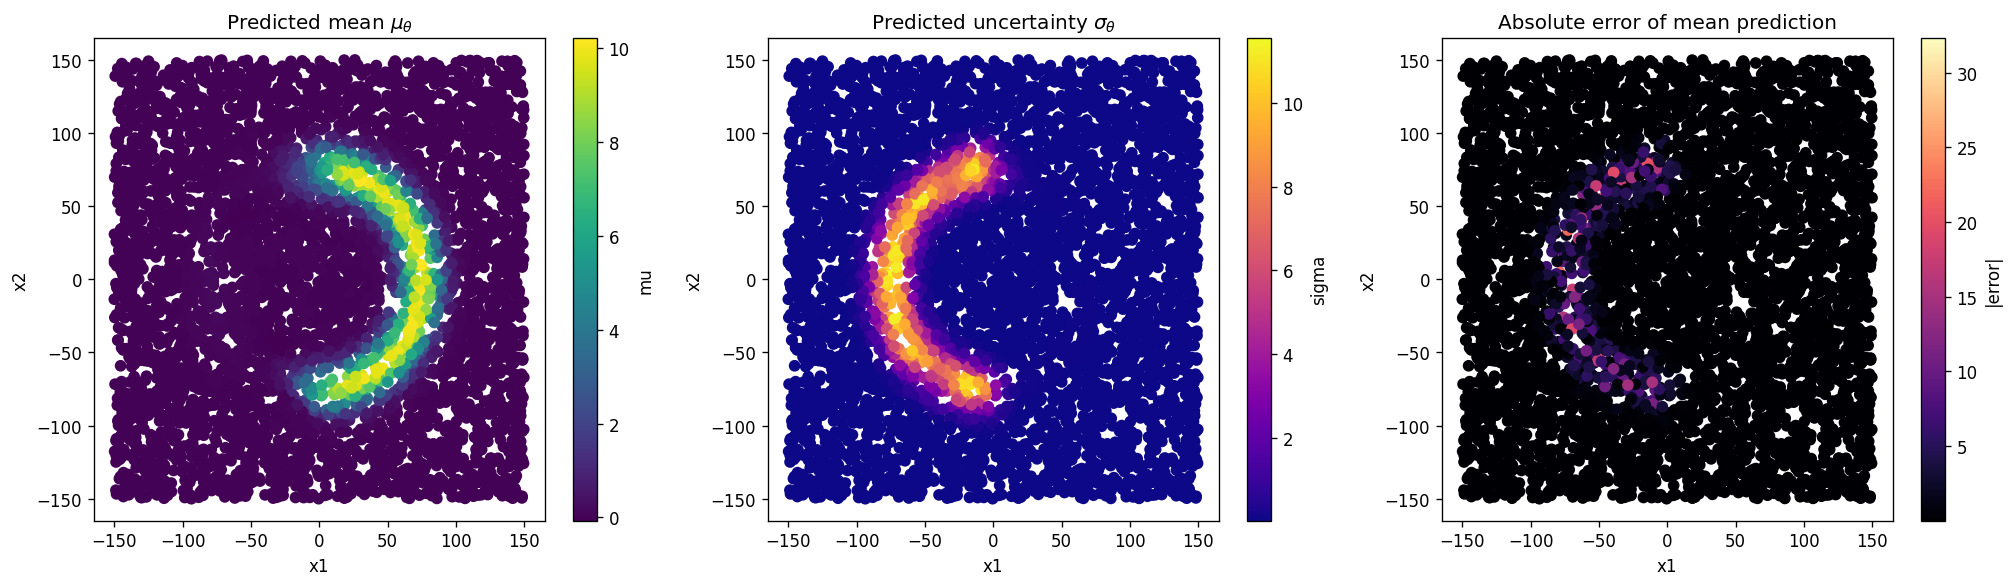
\includegraphics[width=\textwidth]{3.3.4_2.png}
\caption{Predicted mean, predicted uncertainty, and absolute error on the uncertainty dataset.}
\end{figure}

The probabilistic model achieved a test MSE of 3.8097 and an average predicted uncertainty of 0.6463. Its raw MSE was slightly worse than the deterministic model, but it additionally provided meaningful uncertainty estimates. High values of \(\sigma_\theta\) appear mainly in regions where the absolute prediction error is also larger, which indicates that the model learned to associate more difficult samples with higher uncertainty.

% -------------------------------------------------

\subsection*{3.3.5 California Housing with Uncertainty}

\textbf{Task:} Apply the probabilistic model to the California Housing dataset and analyze uncertainty-quality relationships.

\vspace{0.3cm}

\textbf{Results:}

\begin{figure}[H]
\centering
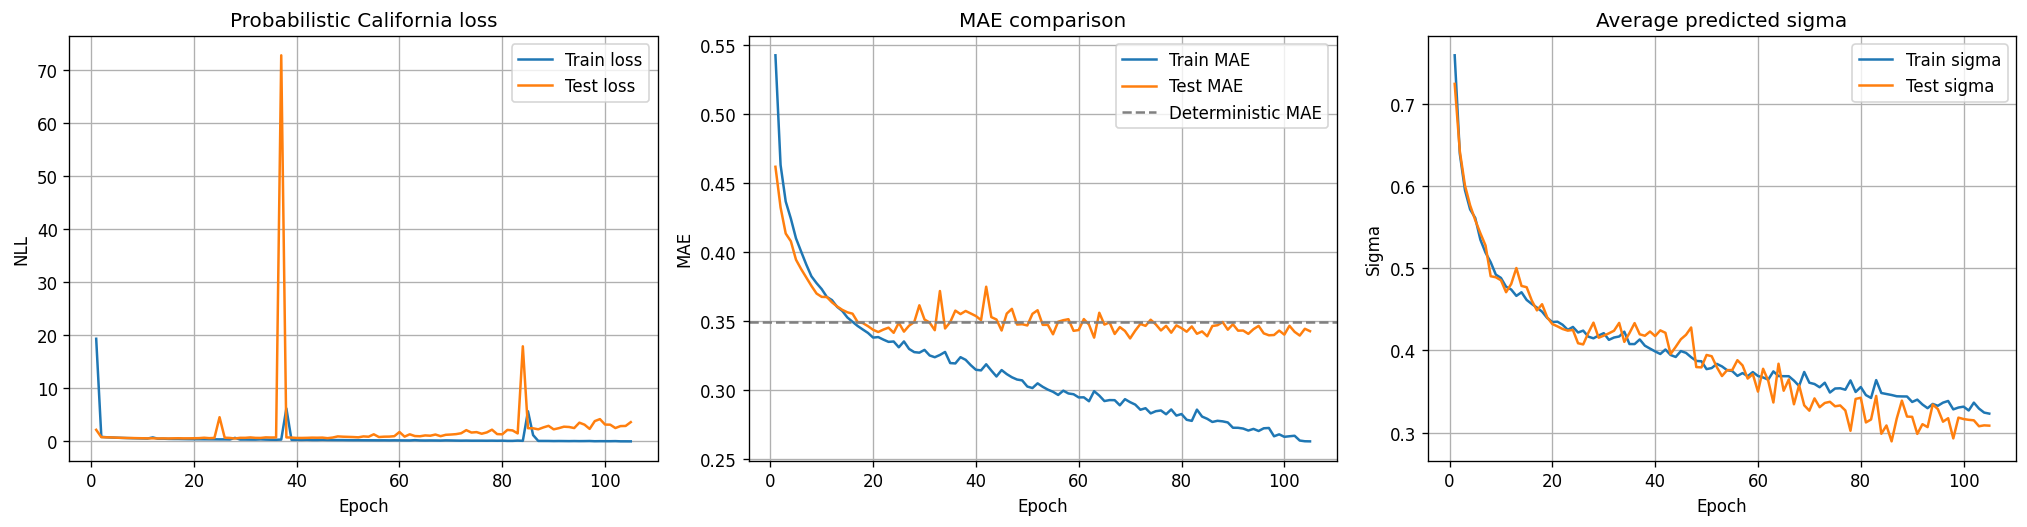
\includegraphics[width=\textwidth]{3.3.5.png}
\caption{Probabilistic California Housing learning curves.}
\end{figure}

\begin{figure}[H]
\centering
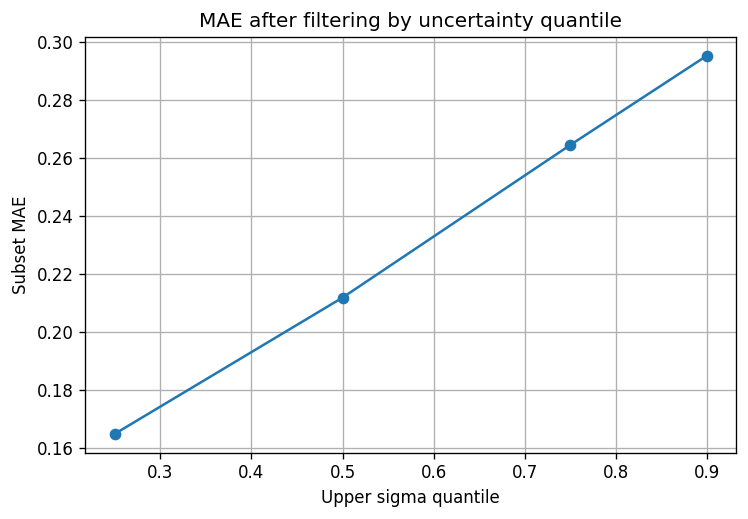
\includegraphics[width=0.7\textwidth]{3.3.5_2.png}
\caption{Subset MAE after filtering predictions by upper uncertainty quantiles.}
\end{figure}

The probabilistic version improved the deterministic California Housing result from 0.3494 to 0.3374 MAE. The correlation coefficient between the absolute prediction error and the predicted uncertainty was 0.2201, which indicates a positive relationship between uncertainty and actual error.

Filtering by uncertainty quantiles produced the following subset MAEs:

\begin{table}[H]
\centering
\caption{MAE after filtering by predicted uncertainty.}
\begin{tabular}{cccc}
\toprule
Upper sigma quantile & Threshold & Subset size & Subset MAE \\
\midrule
0.25 & 0.1707 & 1032 & 0.1649 \\
0.50 & 0.2780 & 2064 & 0.2118 \\
0.75 & 0.4236 & 3096 & 0.2645 \\
0.90 & 0.5770 & 3715 & 0.2953 \\
\bottomrule
\end{tabular}
\end{table}

These results show that the predictions with the smallest estimated uncertainty are substantially more accurate than the full test set average, which confirms that the uncertainty output is useful for ranking prediction quality.

% =================================================
% Problem 3.4
% =================================================

\section*{Problem 3.4}

\subsection*{3.4.1 Gradient Boosting Residuals}

\textbf{Task:} Show that the negative gradient of the squared loss corresponds to residuals.

\vspace{0.3cm}

\textbf{Results:}

For squared loss,

\[
L(y_i,F_{m-1}(x_i)) = (y_i - F_{m-1}(x_i))^2,
\]

the derivative with respect to the current ensemble output is

\[
\frac{\partial L}{\partial F_{m-1}(x_i)}
=
2(F_{m-1}(x_i)-y_i).
\]

Therefore, the negative gradient is

\[
-\nabla_{F_{m-1}} L
=
2(y_i-F_{m-1}(x_i)),
\]

which is equal to the residual up to the constant factor 2. Consequently, each new weak learner is fitted to the current residual structure of the ensemble, which means that every boosting step aims to correct the errors still left by the previous model.

% -------------------------------------------------

\subsection*{3.4.2 Gradient Boosting Regression}

\textbf{Task:} Implement gradient boosting regression using shallow decision trees.

\vspace{0.3cm}

\textbf{Results:}

\begin{figure}[H]
\centering
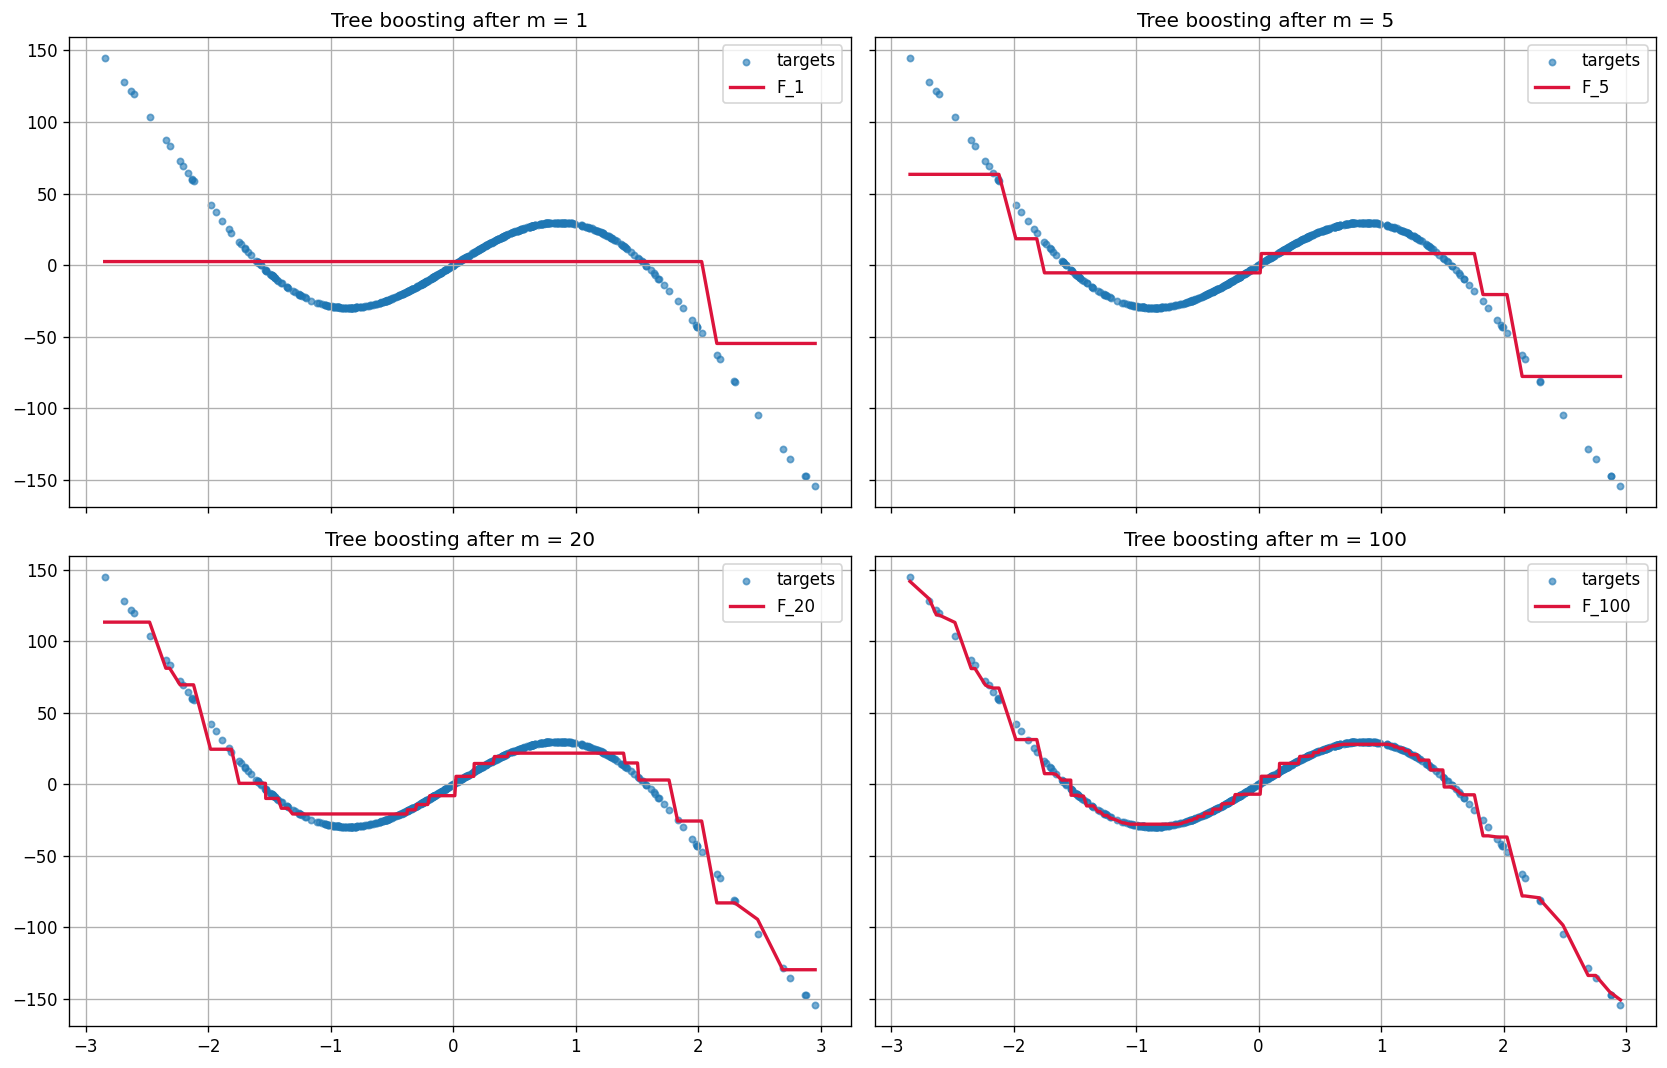
\includegraphics[width=\textwidth]{3.4.2.png}
\caption{Tree-based boosting regressor estimates for increasing ensemble sizes.}
\end{figure}

\begin{figure}[H]
\centering
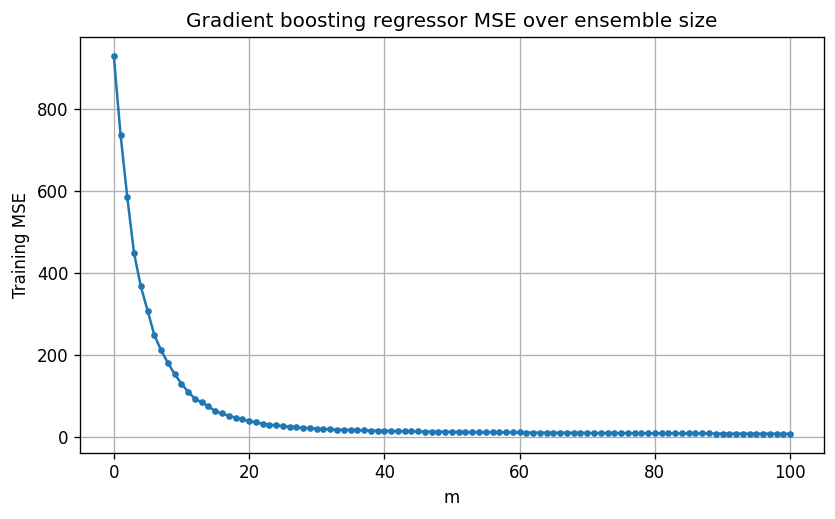
\includegraphics[width=0.75\textwidth]{3.4.2_2.png}
\caption{Training MSE over ensemble size for the tree-based boosting regressor.}
\end{figure}

Using \texttt{DecisionTreeRegressor(max\_depth=1)} as the weak learner and a fixed step size of \(\alpha=0.5\), the boosting model progressively approximated the nonlinear regression target. The final training MSE after \(M=100\) learners was 6.8638. The evolution of the fitted function shows the typical piecewise-constant refinement introduced by decision stumps.

% -------------------------------------------------

\subsection*{3.4.3 Linear Weak Learners}

\textbf{Task:} Replace trees with linear regression weak learners and compare performance.

\vspace{0.3cm}

\textbf{Results:}

\begin{figure}[H]
\centering
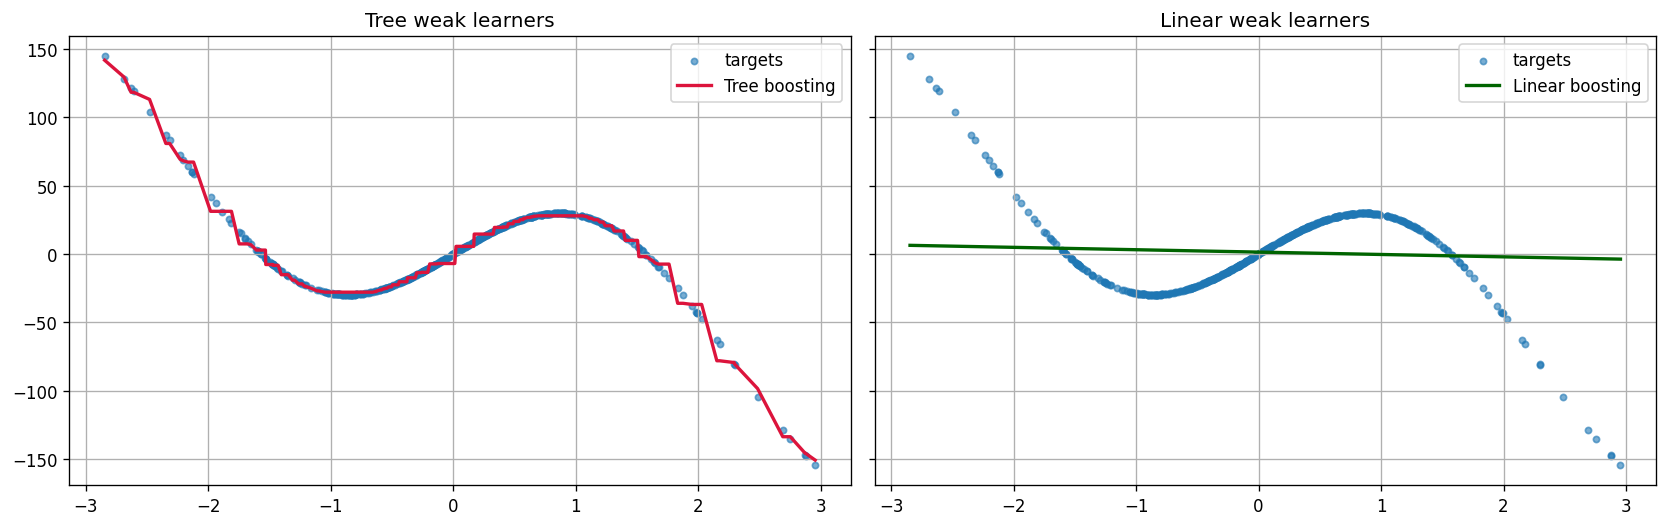
\includegraphics[width=\textwidth]{3.4.3.png}
\caption{Comparison of the final regression fit obtained with tree and linear weak learners.}
\end{figure}

\begin{figure}[H]
\centering
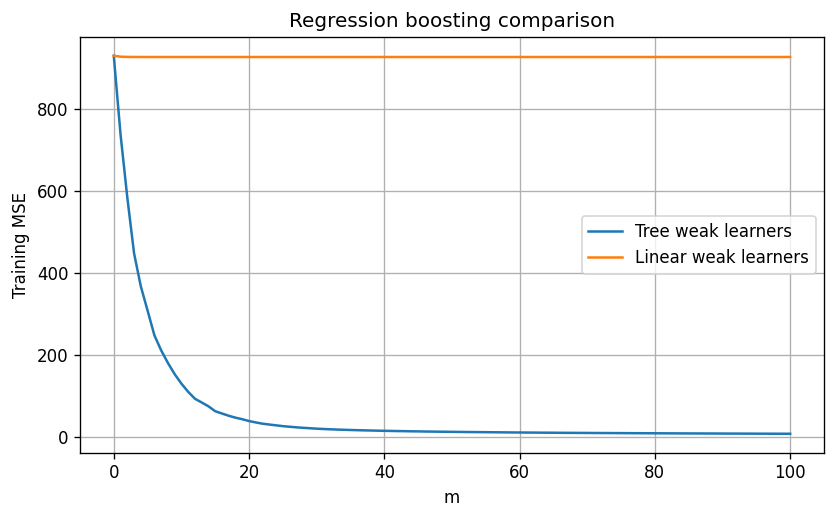
\includegraphics[width=0.75\textwidth]{3.4.3_2.png}
\caption{MSE comparison between tree-based and linear weak learners.}
\end{figure}

The final training MSE with tree weak learners was 6.8638, whereas the corresponding value for linear weak learners was 927.6935. This large gap shows that linear models are far too rigid for this nonlinear residual-fitting task. Tree stumps can apply local corrections in different input regions, while a linear regressor can only add a global affine correction at each stage, which makes it a poor choice here.

% -------------------------------------------------

\subsection*{3.4.4 Cross-Entropy Residuals}

\textbf{Task:} Derive the pseudo-residuals for binary cross-entropy classification.

\vspace{0.3cm}

\textbf{Results:}

For binary classification, the ensemble score \(F\) is mapped to a probability through the sigmoid:

\[
\hat{y} = \sigma(F) = \frac{1}{1+e^{-F}}.
\]

The cross-entropy loss is

\[
L = -(y\log(\hat{y}) + (1-y)\log(1-\hat{y})).
\]

Using the chain rule,

\[
\frac{\partial L}{\partial F}
=
\frac{\partial L}{\partial \hat{y}}
\cdot
\frac{\partial \hat{y}}{\partial F}.
\]

Since

\[
\frac{\partial \hat{y}}{\partial F} = \hat{y}(1-\hat{y}),
\]

the derivative simplifies to

\[
\frac{\partial L}{\partial F} = \hat{y} - y.
\]

Therefore, the negative gradient is

\[
-\frac{\partial L}{\partial F} = y - \hat{y},
\]

which is exactly the pseudo-residual used in binary gradient boosting.

% -------------------------------------------------

\subsection*{3.4.5 Gradient Boosting Classification}

\textbf{Task:} Extend the implementation to binary classification and visualize the decision surface.

\vspace{0.3cm}

\textbf{Results:}

\begin{figure}[H]
\centering
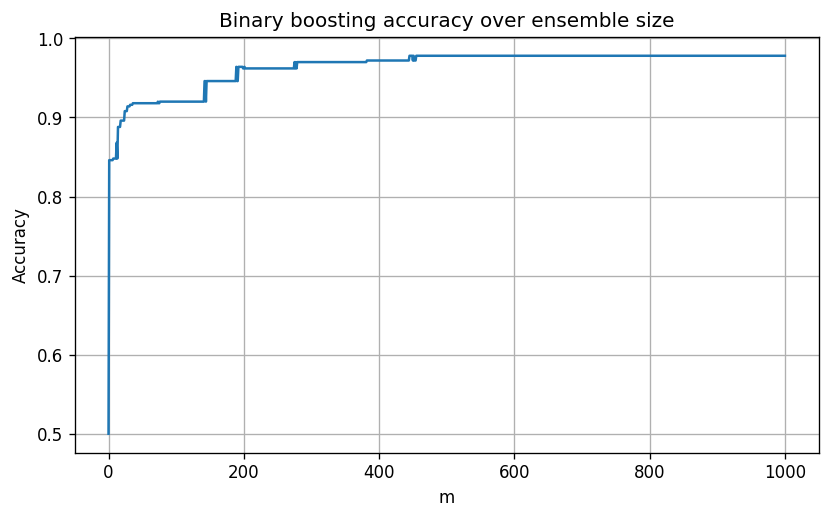
\includegraphics[width=0.75\textwidth]{3.4.5.png}
\caption{Training accuracy over ensemble size for tree-based binary boosting.}
\end{figure}

\begin{figure}[H]
\centering
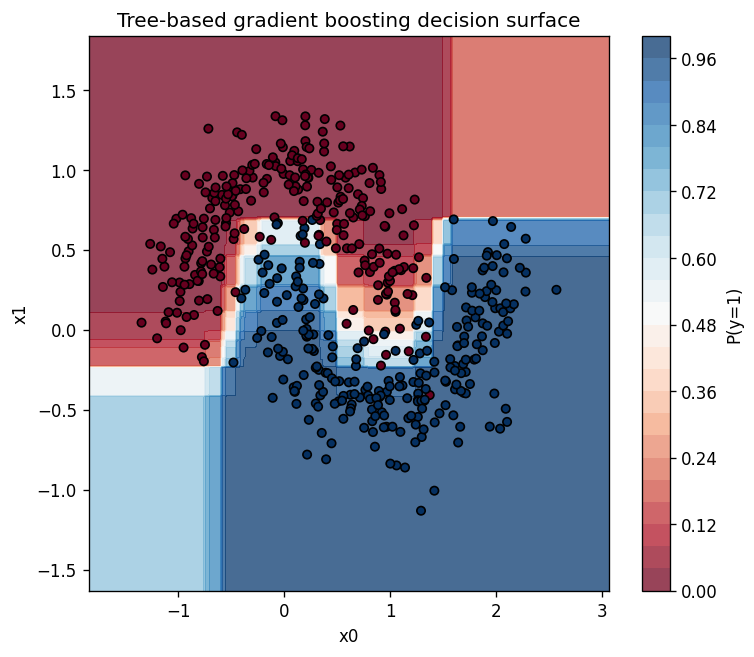
\includegraphics[width=0.7\textwidth]{3.4.5_2.png}
\caption{Decision surface of tree-based binary gradient boosting.}
\end{figure}

The measured accuracies for selected ensemble sizes were:

\begin{table}[H]
\centering
\caption{Binary boosting accuracy with tree weak learners.}
\begin{tabular}{cc}
\toprule
Ensemble size \(m\) & Accuracy \\
\midrule
1 & 0.8460 \\
10 & 0.8480 \\
100 & 0.9200 \\
1000 & 0.9780 \\
\bottomrule
\end{tabular}
\end{table}

The decision surface is highly non-linear and piecewise-constant, which is consistent with the use of decision-tree weak learners. As more learners are added, the classifier progressively sharpens the separation between the two classes.

% -------------------------------------------------

\subsection*{3.4.6 Linear Classification Weak Learners}

\textbf{Task:} Replace trees with linear regression weak learners and compare decision boundaries.

\vspace{0.3cm}

\textbf{Results:}

\begin{figure}[H]
\centering
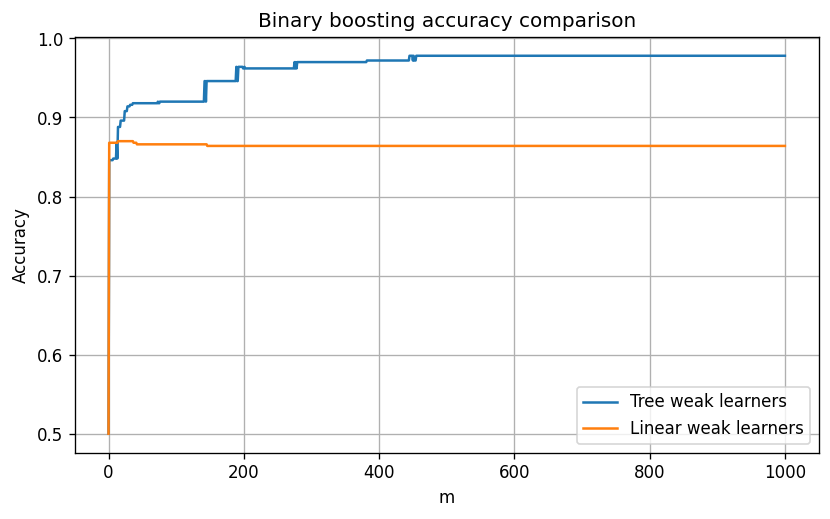
\includegraphics[width=0.75\textwidth]{3.4.6.png}
\caption{Accuracy comparison between tree and linear weak learners for binary boosting.}
\end{figure}

\begin{figure}[H]
\centering
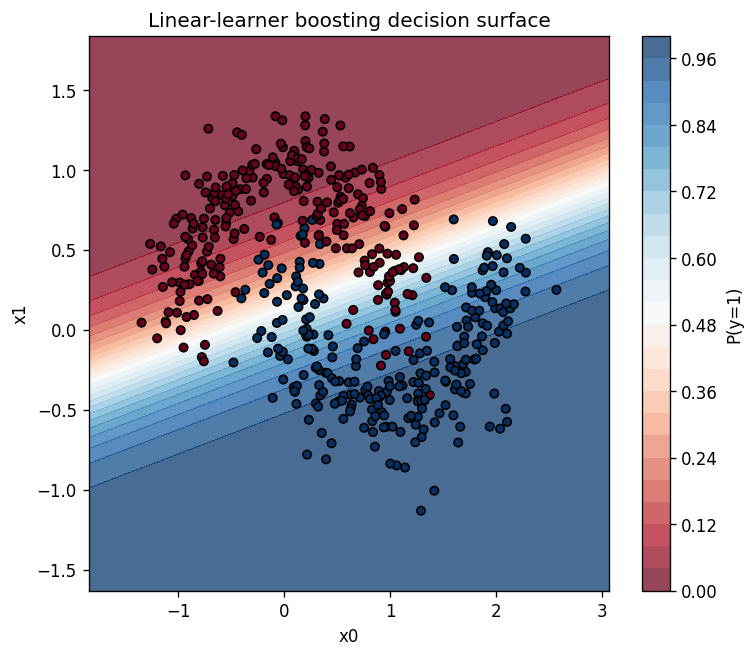
\includegraphics[width=0.7\textwidth]{3.4.6_2.png}
\caption{Decision surface obtained with linear weak learners.}
\end{figure}

The linear-learner accuracies were 0.8680 for \(m=1\), 0.8680 for \(m=10\), 0.8660 for \(m=100\), and 0.8640 for \(m=1000\). The final tree-based model reached 0.9780 accuracy, whereas the linear-learner variant remained at 0.8640.

The linear version produces a much smoother decision boundary, essentially resembling a globally tilted separator. In contrast, tree weak learners create localized piecewise-constant corrections, which makes them much better suited for capturing the nonlinear class structure present in the dataset.

% =================================================

\end{document}